\documentclass[twoside]{book}

% Packages required by doxygen
\usepackage{fixltx2e}
\usepackage{calc}
\usepackage{doxygen}
\usepackage[export]{adjustbox} % also loads graphicx
\usepackage{graphicx}
\usepackage[utf8]{inputenc}
\usepackage{makeidx}
\usepackage{multicol}
\usepackage{multirow}
\PassOptionsToPackage{warn}{textcomp}
\usepackage{textcomp}
\usepackage[nointegrals]{wasysym}
\usepackage[table]{xcolor}

% Font selection
\usepackage[T1]{fontenc}
\usepackage[scaled=.90]{helvet}
\usepackage{courier}
\usepackage{amssymb}
\usepackage{sectsty}
\renewcommand{\familydefault}{\sfdefault}
\allsectionsfont{%
  \fontseries{bc}\selectfont%
  \color{darkgray}%
}
\renewcommand{\DoxyLabelFont}{%
  \fontseries{bc}\selectfont%
  \color{darkgray}%
}
\newcommand{\+}{\discretionary{\mbox{\scriptsize$\hookleftarrow$}}{}{}}

% Page & text layout
\usepackage{geometry}
\geometry{%
  a4paper,%
  top=2.5cm,%
  bottom=2.5cm,%
  left=2.5cm,%
  right=2.5cm%
}
\tolerance=750
\hfuzz=15pt
\hbadness=750
\setlength{\emergencystretch}{15pt}
\setlength{\parindent}{0cm}
\setlength{\parskip}{0.2cm}
\makeatletter
\renewcommand{\paragraph}{%
  \@startsection{paragraph}{4}{0ex}{-1.0ex}{1.0ex}{%
    \normalfont\normalsize\bfseries\SS@parafont%
  }%
}
\renewcommand{\subparagraph}{%
  \@startsection{subparagraph}{5}{0ex}{-1.0ex}{1.0ex}{%
    \normalfont\normalsize\bfseries\SS@subparafont%
  }%
}
\makeatother

% Headers & footers
\usepackage{fancyhdr}
\pagestyle{fancyplain}
\fancyhead[LE]{\fancyplain{}{\bfseries\thepage}}
\fancyhead[CE]{\fancyplain{}{}}
\fancyhead[RE]{\fancyplain{}{\bfseries\leftmark}}
\fancyhead[LO]{\fancyplain{}{\bfseries\rightmark}}
\fancyhead[CO]{\fancyplain{}{}}
\fancyhead[RO]{\fancyplain{}{\bfseries\thepage}}
\fancyfoot[LE]{\fancyplain{}{}}
\fancyfoot[CE]{\fancyplain{}{}}
\fancyfoot[RE]{\fancyplain{}{\bfseries\scriptsize Generated on Tue May 10 2016 21\+:32\+:04 for Group2\+Test\+Project by Doxygen }}
\fancyfoot[LO]{\fancyplain{}{\bfseries\scriptsize Generated on Tue May 10 2016 21\+:32\+:04 for Group2\+Test\+Project by Doxygen }}
\fancyfoot[CO]{\fancyplain{}{}}
\fancyfoot[RO]{\fancyplain{}{}}
\renewcommand{\footrulewidth}{0.4pt}
\renewcommand{\chaptermark}[1]{%
  \markboth{#1}{}%
}
\renewcommand{\sectionmark}[1]{%
  \markright{\thesection\ #1}%
}

% Indices & bibliography
\usepackage{natbib}
\usepackage[titles]{tocloft}
\setcounter{tocdepth}{3}
\setcounter{secnumdepth}{5}
\makeindex

% Hyperlinks (required, but should be loaded last)
\usepackage{ifpdf}
\ifpdf
  \usepackage[pdftex,pagebackref=true]{hyperref}
\else
  \usepackage[ps2pdf,pagebackref=true]{hyperref}
\fi
\hypersetup{%
  colorlinks=true,%
  linkcolor=blue,%
  citecolor=blue,%
  unicode%
}

% Custom commands
\newcommand{\clearemptydoublepage}{%
  \newpage{\pagestyle{empty}\cleardoublepage}%
}


%===== C O N T E N T S =====

\begin{document}

% Titlepage & ToC
\hypersetup{pageanchor=false,
             bookmarks=true,
             bookmarksnumbered=true,
             pdfencoding=unicode
            }
\pagenumbering{roman}
\begin{titlepage}
\vspace*{7cm}
\begin{center}%
{\Large Group2\+Test\+Project }\\
\vspace*{1cm}
{\large Generated by Doxygen 1.8.10}\\
\vspace*{0.5cm}
{\small Tue May 10 2016 21:32:04}\\
\end{center}
\end{titlepage}
\clearemptydoublepage
\tableofcontents
\clearemptydoublepage
\pagenumbering{arabic}
\hypersetup{pageanchor=true}

%--- Begin generated contents ---
\chapter{Hierarchical Index}
\section{Class Hierarchy}
This inheritance list is sorted roughly, but not completely, alphabetically\+:\begin{DoxyCompactList}
\item Http\+Servlet\begin{DoxyCompactList}
\item \contentsline{section}{Arda\+Servlet}{\pageref{class_arda_servlet}}{}
\item \contentsline{section}{Enes\+Servlet}{\pageref{class_enes_servlet}}{}
\item \contentsline{section}{Erkam\+Servlet}{\pageref{class_erkam_servlet}}{}
\item \contentsline{section}{Gozde\+Servlet}{\pageref{class_gozde_servlet}}{}
\item \contentsline{section}{Kagan\+Servlet}{\pageref{class_kagan_servlet}}{}
\item \contentsline{section}{Main\+Page\+Servlet}{\pageref{class_main_page_servlet}}{}
\item \contentsline{section}{Osman\+Servlet}{\pageref{class_osman_servlet}}{}
\item \contentsline{section}{Yigit\+Servlet}{\pageref{class_yigit_servlet}}{}
\end{DoxyCompactList}
\end{DoxyCompactList}

\chapter{Class Index}
\section{Class List}
Here are the classes, structs, unions and interfaces with brief descriptions\+:\begin{DoxyCompactList}
\item\contentsline{section}{\hyperlink{classdeneme_1_1_db}{deneme.\+Db} }{\pageref{classdeneme_1_1_db}}{}
\item\contentsline{section}{\hyperlink{classdeneme_1_1_delete_servlet}{deneme.\+Delete\+Servlet} }{\pageref{classdeneme_1_1_delete_servlet}}{}
\item\contentsline{section}{\hyperlink{classdeneme_1_1_enes_servlet}{deneme.\+Enes\+Servlet} }{\pageref{classdeneme_1_1_enes_servlet}}{}
\item\contentsline{section}{\hyperlink{classdeneme_1_1_sparql}{deneme.\+Sparql} }{\pageref{classdeneme_1_1_sparql}}{}
\end{DoxyCompactList}

\chapter{Class Documentation}
\hypertarget{class_arda_servlet}{}\section{Arda\+Servlet Class Reference}
\label{class_arda_servlet}\index{Arda\+Servlet@{Arda\+Servlet}}
Inheritance diagram for Arda\+Servlet\+:\begin{figure}[H]
\begin{center}
\leavevmode
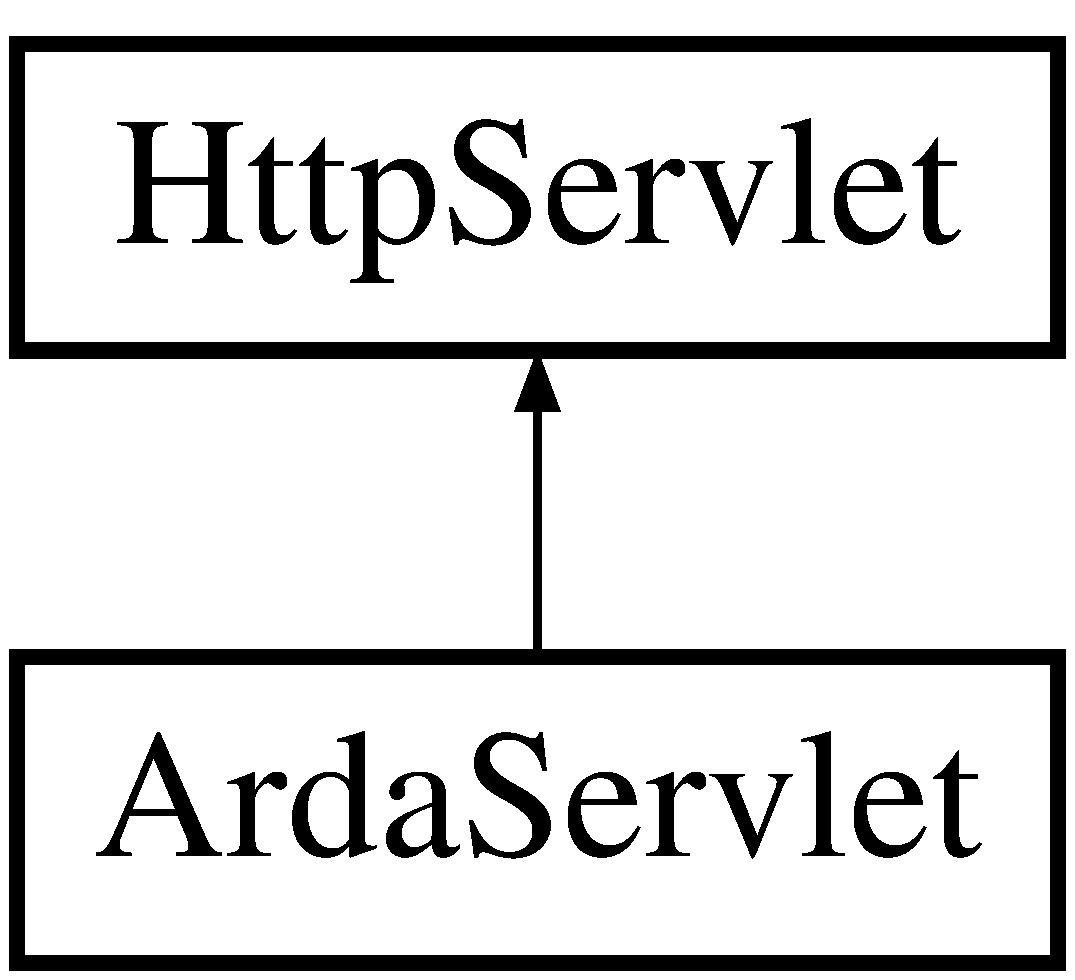
\includegraphics[height=2.000000cm]{class_arda_servlet}
\end{center}
\end{figure}
\subsection*{Public Member Functions}
\begin{DoxyCompactItemize}
\item 
\hyperlink{class_arda_servlet_a2c6a6ef64e38c420227933a842db3363}{Arda\+Servlet} ()
\end{DoxyCompactItemize}
\subsection*{Protected Member Functions}
\begin{DoxyCompactItemize}
\item 
void \hyperlink{class_arda_servlet_a243cd4607430d73826f59a340b04a7a5}{do\+Get} (Http\+Servlet\+Request request, Http\+Servlet\+Response response)  throws Servlet\+Exception, I\+O\+Exception 
\item 
void \hyperlink{class_arda_servlet_a327279374b3d8a0a283b8e3b7c1ce739}{do\+Post} (Http\+Servlet\+Request request, Http\+Servlet\+Response response)  throws Servlet\+Exception, I\+O\+Exception 
\end{DoxyCompactItemize}


\subsection{Detailed Description}
Servlet implementation class \hyperlink{class_arda_servlet}{Arda\+Servlet} 

\subsection{Constructor \& Destructor Documentation}
\hypertarget{class_arda_servlet_a2c6a6ef64e38c420227933a842db3363}{}\index{Arda\+Servlet@{Arda\+Servlet}!Arda\+Servlet@{Arda\+Servlet}}
\index{Arda\+Servlet@{Arda\+Servlet}!Arda\+Servlet@{Arda\+Servlet}}
\subsubsection[{Arda\+Servlet()}]{\setlength{\rightskip}{0pt plus 5cm}Arda\+Servlet.\+Arda\+Servlet (
\begin{DoxyParamCaption}
{}
\end{DoxyParamCaption}
)}\label{class_arda_servlet_a2c6a6ef64e38c420227933a842db3363}
\begin{DoxySeeAlso}{See also}
Http\+Servlet\+::\+Http\+Servlet() 
\end{DoxySeeAlso}


\subsection{Member Function Documentation}
\hypertarget{class_arda_servlet_a243cd4607430d73826f59a340b04a7a5}{}\index{Arda\+Servlet@{Arda\+Servlet}!do\+Get@{do\+Get}}
\index{do\+Get@{do\+Get}!Arda\+Servlet@{Arda\+Servlet}}
\subsubsection[{do\+Get(\+Http\+Servlet\+Request request, Http\+Servlet\+Response response)}]{\setlength{\rightskip}{0pt plus 5cm}void Arda\+Servlet.\+do\+Get (
\begin{DoxyParamCaption}
\item[{Http\+Servlet\+Request}]{request, }
\item[{Http\+Servlet\+Response}]{response}
\end{DoxyParamCaption}
) throws Servlet\+Exception, I\+O\+Exception\hspace{0.3cm}{\ttfamily [protected]}}\label{class_arda_servlet_a243cd4607430d73826f59a340b04a7a5}
\begin{DoxySeeAlso}{See also}
Http\+Servlet\+::do\+Get(\+Http\+Servlet\+Request request, Http\+Servlet\+Response response) 
\end{DoxySeeAlso}
\hypertarget{class_arda_servlet_a327279374b3d8a0a283b8e3b7c1ce739}{}\index{Arda\+Servlet@{Arda\+Servlet}!do\+Post@{do\+Post}}
\index{do\+Post@{do\+Post}!Arda\+Servlet@{Arda\+Servlet}}
\subsubsection[{do\+Post(\+Http\+Servlet\+Request request, Http\+Servlet\+Response response)}]{\setlength{\rightskip}{0pt plus 5cm}void Arda\+Servlet.\+do\+Post (
\begin{DoxyParamCaption}
\item[{Http\+Servlet\+Request}]{request, }
\item[{Http\+Servlet\+Response}]{response}
\end{DoxyParamCaption}
) throws Servlet\+Exception, I\+O\+Exception\hspace{0.3cm}{\ttfamily [protected]}}\label{class_arda_servlet_a327279374b3d8a0a283b8e3b7c1ce739}
\begin{DoxySeeAlso}{See also}
Http\+Servlet\+::do\+Post(\+Http\+Servlet\+Request request, Http\+Servlet\+Response response) 
\end{DoxySeeAlso}


The documentation for this class was generated from the following file\+:\begin{DoxyCompactItemize}
\item 
src/Arda\+Servlet.\+java\end{DoxyCompactItemize}

\hypertarget{class_enes_servlet}{}\section{Enes\+Servlet Class Reference}
\label{class_enes_servlet}\index{Enes\+Servlet@{Enes\+Servlet}}
Inheritance diagram for Enes\+Servlet\+:\begin{figure}[H]
\begin{center}
\leavevmode
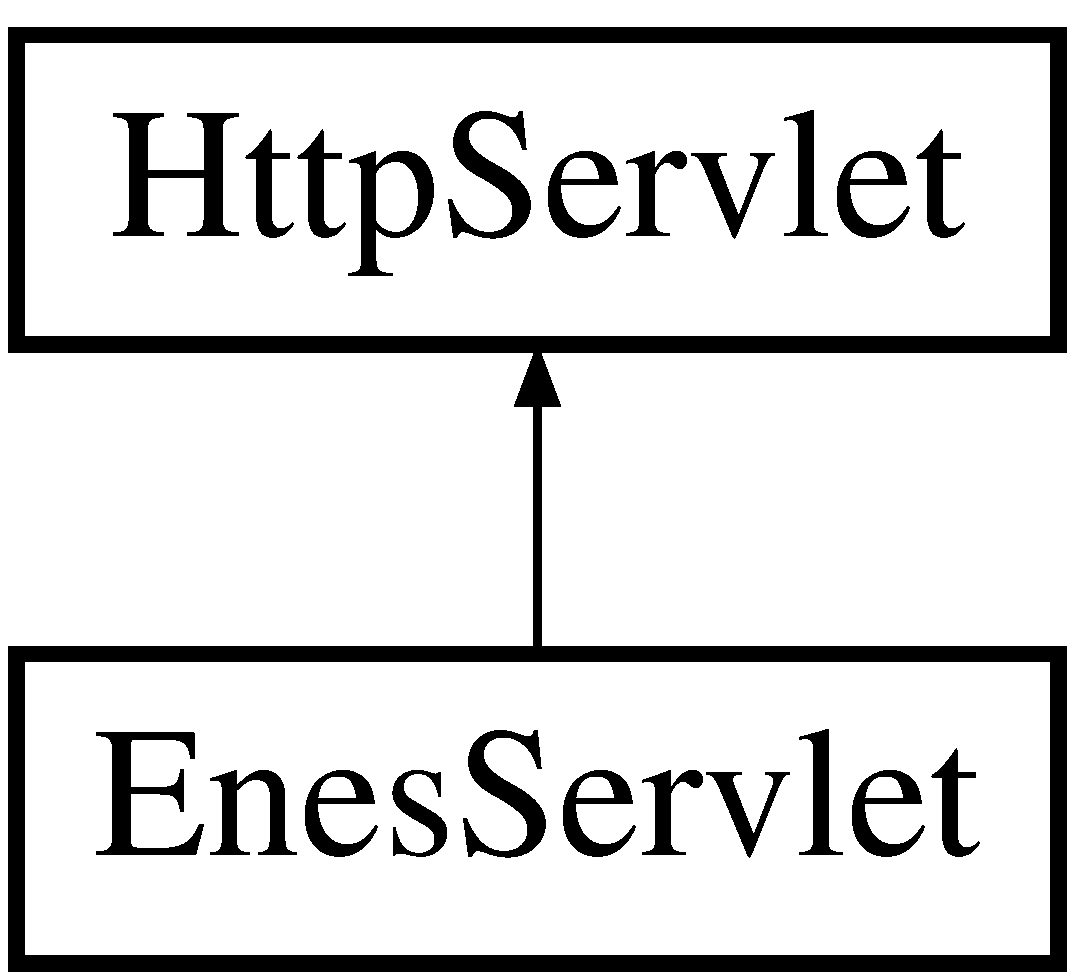
\includegraphics[height=2.000000cm]{class_enes_servlet}
\end{center}
\end{figure}
\subsection*{Public Member Functions}
\begin{DoxyCompactItemize}
\item 
\hyperlink{class_enes_servlet_ab2c4a798526e86540e90c65ee48fa081}{Enes\+Servlet} ()
\end{DoxyCompactItemize}
\subsection*{Protected Member Functions}
\begin{DoxyCompactItemize}
\item 
void \hyperlink{class_enes_servlet_aa6af381d4229895e07a125b9342e71a1}{do\+Get} (Http\+Servlet\+Request request, Http\+Servlet\+Response response)  throws Servlet\+Exception, I\+O\+Exception 
\item 
void \hyperlink{class_enes_servlet_a438292b768bc1ff3606769e3a0b8b397}{do\+Post} (Http\+Servlet\+Request request, Http\+Servlet\+Response response)  throws Servlet\+Exception, I\+O\+Exception 
\end{DoxyCompactItemize}


\subsection{Detailed Description}
Servlet implementation class \hyperlink{class_enes_servlet}{Enes\+Servlet} 

\subsection{Constructor \& Destructor Documentation}
\hypertarget{class_enes_servlet_ab2c4a798526e86540e90c65ee48fa081}{}\index{Enes\+Servlet@{Enes\+Servlet}!Enes\+Servlet@{Enes\+Servlet}}
\index{Enes\+Servlet@{Enes\+Servlet}!Enes\+Servlet@{Enes\+Servlet}}
\subsubsection[{Enes\+Servlet()}]{\setlength{\rightskip}{0pt plus 5cm}Enes\+Servlet.\+Enes\+Servlet (
\begin{DoxyParamCaption}
{}
\end{DoxyParamCaption}
)}\label{class_enes_servlet_ab2c4a798526e86540e90c65ee48fa081}
\begin{DoxySeeAlso}{See also}
Http\+Servlet\+::\+Http\+Servlet() 
\end{DoxySeeAlso}


\subsection{Member Function Documentation}
\hypertarget{class_enes_servlet_aa6af381d4229895e07a125b9342e71a1}{}\index{Enes\+Servlet@{Enes\+Servlet}!do\+Get@{do\+Get}}
\index{do\+Get@{do\+Get}!Enes\+Servlet@{Enes\+Servlet}}
\subsubsection[{do\+Get(\+Http\+Servlet\+Request request, Http\+Servlet\+Response response)}]{\setlength{\rightskip}{0pt plus 5cm}void Enes\+Servlet.\+do\+Get (
\begin{DoxyParamCaption}
\item[{Http\+Servlet\+Request}]{request, }
\item[{Http\+Servlet\+Response}]{response}
\end{DoxyParamCaption}
) throws Servlet\+Exception, I\+O\+Exception\hspace{0.3cm}{\ttfamily [protected]}}\label{class_enes_servlet_aa6af381d4229895e07a125b9342e71a1}
\begin{DoxySeeAlso}{See also}
Http\+Servlet\+::do\+Get(\+Http\+Servlet\+Request request, Http\+Servlet\+Response response) 
\end{DoxySeeAlso}
\hypertarget{class_enes_servlet_a438292b768bc1ff3606769e3a0b8b397}{}\index{Enes\+Servlet@{Enes\+Servlet}!do\+Post@{do\+Post}}
\index{do\+Post@{do\+Post}!Enes\+Servlet@{Enes\+Servlet}}
\subsubsection[{do\+Post(\+Http\+Servlet\+Request request, Http\+Servlet\+Response response)}]{\setlength{\rightskip}{0pt plus 5cm}void Enes\+Servlet.\+do\+Post (
\begin{DoxyParamCaption}
\item[{Http\+Servlet\+Request}]{request, }
\item[{Http\+Servlet\+Response}]{response}
\end{DoxyParamCaption}
) throws Servlet\+Exception, I\+O\+Exception\hspace{0.3cm}{\ttfamily [protected]}}\label{class_enes_servlet_a438292b768bc1ff3606769e3a0b8b397}
\begin{DoxySeeAlso}{See also}
Http\+Servlet\+::do\+Post(\+Http\+Servlet\+Request request, Http\+Servlet\+Response response) 
\end{DoxySeeAlso}


The documentation for this class was generated from the following file\+:\begin{DoxyCompactItemize}
\item 
src/Enes\+Servlet.\+java\end{DoxyCompactItemize}

\hypertarget{class_erkam_servlet}{}\section{Erkam\+Servlet Class Reference}
\label{class_erkam_servlet}\index{Erkam\+Servlet@{Erkam\+Servlet}}
Inheritance diagram for Erkam\+Servlet\+:\begin{figure}[H]
\begin{center}
\leavevmode
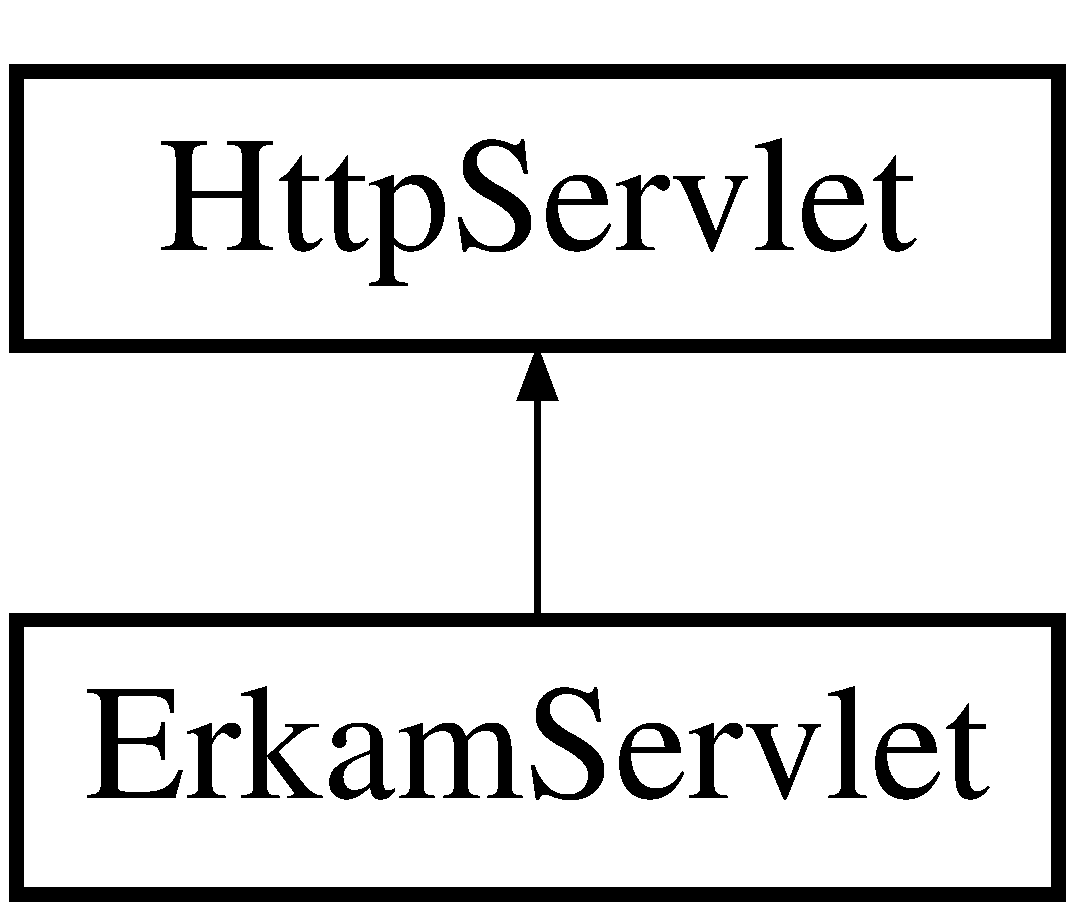
\includegraphics[height=2.000000cm]{class_erkam_servlet}
\end{center}
\end{figure}
\subsection*{Public Member Functions}
\begin{DoxyCompactItemize}
\item 
\hyperlink{class_erkam_servlet_a09f82dd182d218612d4c9c1d1019630b}{Erkam\+Servlet} ()
\end{DoxyCompactItemize}
\subsection*{Protected Member Functions}
\begin{DoxyCompactItemize}
\item 
void \hyperlink{class_erkam_servlet_acdeaf32ac42af0153d7504714b4406cb}{do\+Get} (Http\+Servlet\+Request request, Http\+Servlet\+Response response)  throws Servlet\+Exception, I\+O\+Exception 
\item 
void \hyperlink{class_erkam_servlet_a610c3680c6190db04f6637da6d642d2b}{do\+Post} (Http\+Servlet\+Request request, Http\+Servlet\+Response response)  throws Servlet\+Exception, I\+O\+Exception 
\end{DoxyCompactItemize}


\subsection{Detailed Description}
Servlet implementation class \hyperlink{class_erkam_servlet}{Erkam\+Servlet} 

\subsection{Constructor \& Destructor Documentation}
\hypertarget{class_erkam_servlet_a09f82dd182d218612d4c9c1d1019630b}{}\index{Erkam\+Servlet@{Erkam\+Servlet}!Erkam\+Servlet@{Erkam\+Servlet}}
\index{Erkam\+Servlet@{Erkam\+Servlet}!Erkam\+Servlet@{Erkam\+Servlet}}
\subsubsection[{Erkam\+Servlet()}]{\setlength{\rightskip}{0pt plus 5cm}Erkam\+Servlet.\+Erkam\+Servlet (
\begin{DoxyParamCaption}
{}
\end{DoxyParamCaption}
)}\label{class_erkam_servlet_a09f82dd182d218612d4c9c1d1019630b}
\begin{DoxySeeAlso}{See also}
Http\+Servlet\+::\+Http\+Servlet() 
\end{DoxySeeAlso}


\subsection{Member Function Documentation}
\hypertarget{class_erkam_servlet_acdeaf32ac42af0153d7504714b4406cb}{}\index{Erkam\+Servlet@{Erkam\+Servlet}!do\+Get@{do\+Get}}
\index{do\+Get@{do\+Get}!Erkam\+Servlet@{Erkam\+Servlet}}
\subsubsection[{do\+Get(\+Http\+Servlet\+Request request, Http\+Servlet\+Response response)}]{\setlength{\rightskip}{0pt plus 5cm}void Erkam\+Servlet.\+do\+Get (
\begin{DoxyParamCaption}
\item[{Http\+Servlet\+Request}]{request, }
\item[{Http\+Servlet\+Response}]{response}
\end{DoxyParamCaption}
) throws Servlet\+Exception, I\+O\+Exception\hspace{0.3cm}{\ttfamily [protected]}}\label{class_erkam_servlet_acdeaf32ac42af0153d7504714b4406cb}
\begin{DoxySeeAlso}{See also}
Http\+Servlet\+::do\+Get(\+Http\+Servlet\+Request request, Http\+Servlet\+Response response) 
\end{DoxySeeAlso}
\hypertarget{class_erkam_servlet_a610c3680c6190db04f6637da6d642d2b}{}\index{Erkam\+Servlet@{Erkam\+Servlet}!do\+Post@{do\+Post}}
\index{do\+Post@{do\+Post}!Erkam\+Servlet@{Erkam\+Servlet}}
\subsubsection[{do\+Post(\+Http\+Servlet\+Request request, Http\+Servlet\+Response response)}]{\setlength{\rightskip}{0pt plus 5cm}void Erkam\+Servlet.\+do\+Post (
\begin{DoxyParamCaption}
\item[{Http\+Servlet\+Request}]{request, }
\item[{Http\+Servlet\+Response}]{response}
\end{DoxyParamCaption}
) throws Servlet\+Exception, I\+O\+Exception\hspace{0.3cm}{\ttfamily [protected]}}\label{class_erkam_servlet_a610c3680c6190db04f6637da6d642d2b}
\begin{DoxySeeAlso}{See also}
Http\+Servlet\+::do\+Post(\+Http\+Servlet\+Request request, Http\+Servlet\+Response response) 
\end{DoxySeeAlso}


The documentation for this class was generated from the following file\+:\begin{DoxyCompactItemize}
\item 
src/Erkam\+Servlet.\+java\end{DoxyCompactItemize}

\hypertarget{class_gozde_servlet}{}\section{Gozde\+Servlet Class Reference}
\label{class_gozde_servlet}\index{Gozde\+Servlet@{Gozde\+Servlet}}
Inheritance diagram for Gozde\+Servlet\+:\begin{figure}[H]
\begin{center}
\leavevmode
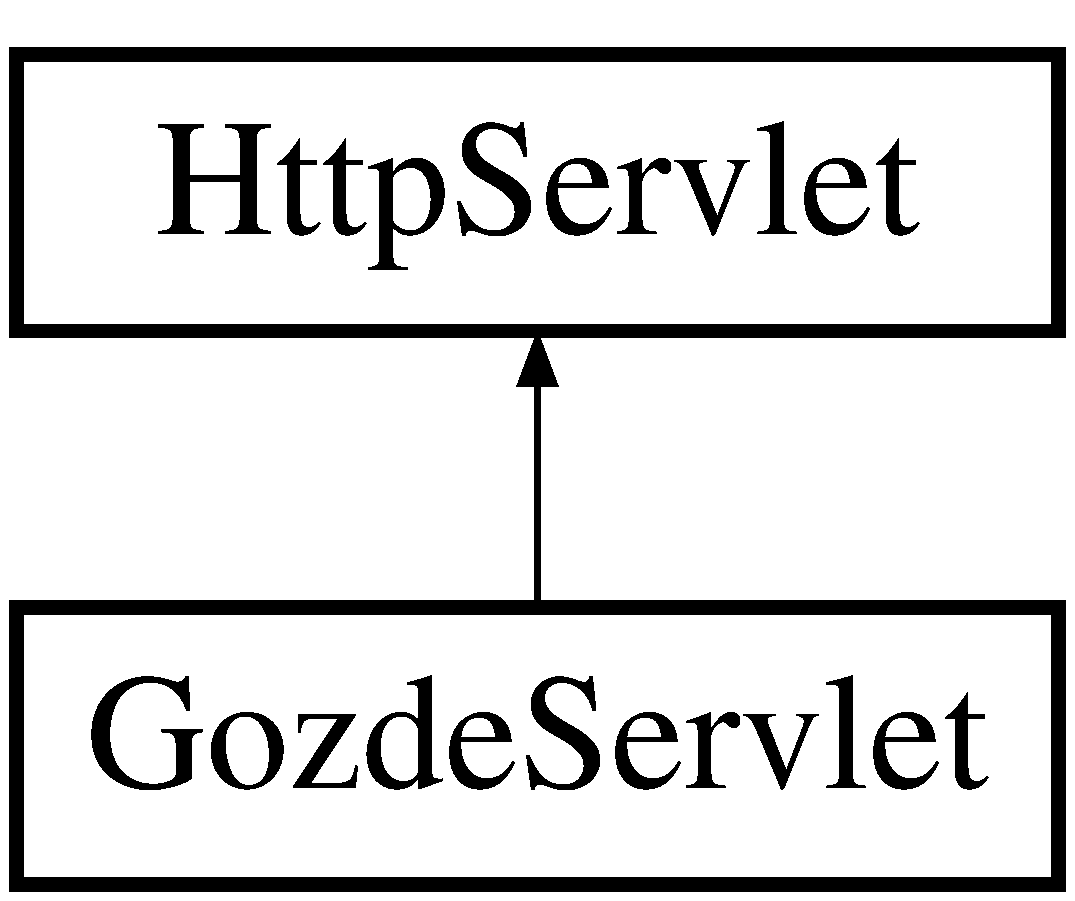
\includegraphics[height=2.000000cm]{class_gozde_servlet}
\end{center}
\end{figure}
\subsection*{Public Member Functions}
\begin{DoxyCompactItemize}
\item 
\hyperlink{class_gozde_servlet_a33fd50df42a07c8b6f1155d084f661ca}{Gozde\+Servlet} ()
\end{DoxyCompactItemize}
\subsection*{Protected Member Functions}
\begin{DoxyCompactItemize}
\item 
void \hyperlink{class_gozde_servlet_acb63c2b11dd710bc124d6eeb89e435ca}{do\+Get} (Http\+Servlet\+Request request, Http\+Servlet\+Response response)  throws Servlet\+Exception, I\+O\+Exception 
\item 
void \hyperlink{class_gozde_servlet_a229714dc005134976cd60c59c20d84c8}{do\+Post} (Http\+Servlet\+Request request, Http\+Servlet\+Response response)  throws Servlet\+Exception, I\+O\+Exception 
\end{DoxyCompactItemize}


\subsection{Detailed Description}
Servlet implementation class \hyperlink{class_gozde_servlet}{Gozde\+Servlet} 

\subsection{Constructor \& Destructor Documentation}
\hypertarget{class_gozde_servlet_a33fd50df42a07c8b6f1155d084f661ca}{}\index{Gozde\+Servlet@{Gozde\+Servlet}!Gozde\+Servlet@{Gozde\+Servlet}}
\index{Gozde\+Servlet@{Gozde\+Servlet}!Gozde\+Servlet@{Gozde\+Servlet}}
\subsubsection[{Gozde\+Servlet()}]{\setlength{\rightskip}{0pt plus 5cm}Gozde\+Servlet.\+Gozde\+Servlet (
\begin{DoxyParamCaption}
{}
\end{DoxyParamCaption}
)}\label{class_gozde_servlet_a33fd50df42a07c8b6f1155d084f661ca}
\begin{DoxySeeAlso}{See also}
Http\+Servlet\+::\+Http\+Servlet() 
\end{DoxySeeAlso}


\subsection{Member Function Documentation}
\hypertarget{class_gozde_servlet_acb63c2b11dd710bc124d6eeb89e435ca}{}\index{Gozde\+Servlet@{Gozde\+Servlet}!do\+Get@{do\+Get}}
\index{do\+Get@{do\+Get}!Gozde\+Servlet@{Gozde\+Servlet}}
\subsubsection[{do\+Get(\+Http\+Servlet\+Request request, Http\+Servlet\+Response response)}]{\setlength{\rightskip}{0pt plus 5cm}void Gozde\+Servlet.\+do\+Get (
\begin{DoxyParamCaption}
\item[{Http\+Servlet\+Request}]{request, }
\item[{Http\+Servlet\+Response}]{response}
\end{DoxyParamCaption}
) throws Servlet\+Exception, I\+O\+Exception\hspace{0.3cm}{\ttfamily [protected]}}\label{class_gozde_servlet_acb63c2b11dd710bc124d6eeb89e435ca}
\begin{DoxySeeAlso}{See also}
Http\+Servlet\+::do\+Get(\+Http\+Servlet\+Request request, Http\+Servlet\+Response response) 
\end{DoxySeeAlso}
\hypertarget{class_gozde_servlet_a229714dc005134976cd60c59c20d84c8}{}\index{Gozde\+Servlet@{Gozde\+Servlet}!do\+Post@{do\+Post}}
\index{do\+Post@{do\+Post}!Gozde\+Servlet@{Gozde\+Servlet}}
\subsubsection[{do\+Post(\+Http\+Servlet\+Request request, Http\+Servlet\+Response response)}]{\setlength{\rightskip}{0pt plus 5cm}void Gozde\+Servlet.\+do\+Post (
\begin{DoxyParamCaption}
\item[{Http\+Servlet\+Request}]{request, }
\item[{Http\+Servlet\+Response}]{response}
\end{DoxyParamCaption}
) throws Servlet\+Exception, I\+O\+Exception\hspace{0.3cm}{\ttfamily [protected]}}\label{class_gozde_servlet_a229714dc005134976cd60c59c20d84c8}
\begin{DoxySeeAlso}{See also}
Http\+Servlet\+::do\+Post(\+Http\+Servlet\+Request request, Http\+Servlet\+Response response) 
\end{DoxySeeAlso}


The documentation for this class was generated from the following file\+:\begin{DoxyCompactItemize}
\item 
src/Gozde\+Servlet.\+java\end{DoxyCompactItemize}

\hypertarget{class_kagan_servlet}{}\section{Kagan\+Servlet Class Reference}
\label{class_kagan_servlet}\index{Kagan\+Servlet@{Kagan\+Servlet}}
Inheritance diagram for Kagan\+Servlet\+:\begin{figure}[H]
\begin{center}
\leavevmode
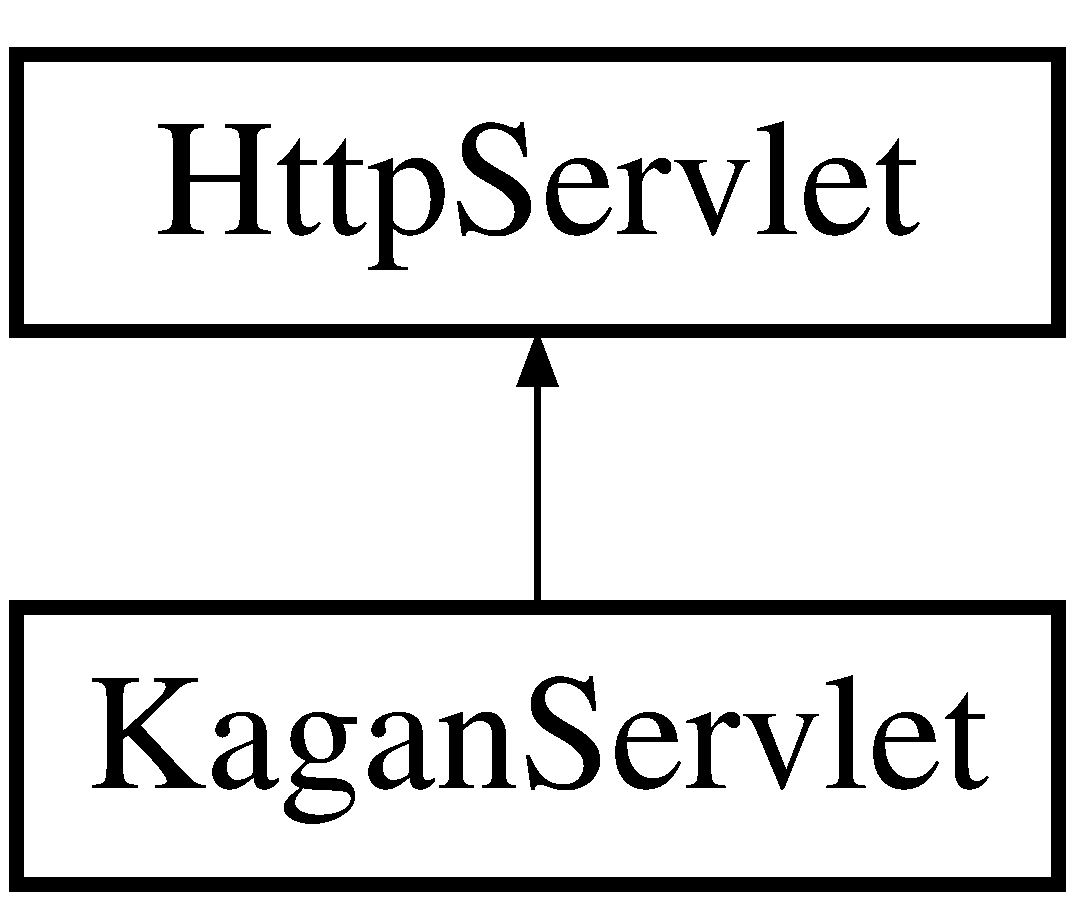
\includegraphics[height=2.000000cm]{class_kagan_servlet}
\end{center}
\end{figure}
\subsection*{Public Member Functions}
\begin{DoxyCompactItemize}
\item 
\hyperlink{class_kagan_servlet_aa9733d9af94d7f9e4fd26e7d4dddca59}{Kagan\+Servlet} ()
\end{DoxyCompactItemize}
\subsection*{Public Attributes}
\begin{DoxyCompactItemize}
\item 
\hypertarget{class_kagan_servlet_abb3da60d4385e88b231d42c79d3c6c0c}{}int {\bfseries radius} = 1\label{class_kagan_servlet_abb3da60d4385e88b231d42c79d3c6c0c}

\item 
\hypertarget{class_kagan_servlet_a59cd96b1ff9052d22081eaa587f295fa}{}int {\bfseries x\+Diff} = 0\label{class_kagan_servlet_a59cd96b1ff9052d22081eaa587f295fa}

\item 
\hypertarget{class_kagan_servlet_a4078c0c4a4dcd1142ab23466b6ea0e68}{}int {\bfseries y\+Diff} = 0\label{class_kagan_servlet_a4078c0c4a4dcd1142ab23466b6ea0e68}

\end{DoxyCompactItemize}
\subsection*{Protected Member Functions}
\begin{DoxyCompactItemize}
\item 
\hypertarget{class_kagan_servlet_ae9cf99b19633877773e6f8346ed44948}{}Connection {\bfseries get\+D\+B\+Connection} ()\label{class_kagan_servlet_ae9cf99b19633877773e6f8346ed44948}

\item 
\hypertarget{class_kagan_servlet_a92634e1d189fec896f1b17e76d9f7043}{}void {\bfseries assign\+Parameters} (Http\+Servlet\+Request request)\label{class_kagan_servlet_a92634e1d189fec896f1b17e76d9f7043}

\item 
\hypertarget{class_kagan_servlet_a051d2f1b8de4f546c7503d422c3d4b13}{}void {\bfseries adjust\+Coordinates} ()\label{class_kagan_servlet_a051d2f1b8de4f546c7503d422c3d4b13}

\item 
\hypertarget{class_kagan_servlet_acb53e6d12a99ea9fe204400e279f5e4e}{}String {\bfseries get\+Query\+String} ()  throws Unsupported\+Encoding\+Exception \label{class_kagan_servlet_acb53e6d12a99ea9fe204400e279f5e4e}

\item 
\hypertarget{class_kagan_servlet_aa741ef72c6695ada00629566c9b5d5cd}{}J\+S\+O\+N\+Array {\bfseries get\+Items} ()  throws I\+O\+Exception, Parse\+Exception \label{class_kagan_servlet_aa741ef72c6695ada00629566c9b5d5cd}

\item 
void \hyperlink{class_kagan_servlet_a069884122c17967444f59c24436e0713}{do\+Get} (Http\+Servlet\+Request request, Http\+Servlet\+Response response)  throws Servlet\+Exception, I\+O\+Exception 
\item 
void \hyperlink{class_kagan_servlet_a557149953b3b57dc5a405506e8349609}{do\+Post} (Http\+Servlet\+Request request, Http\+Servlet\+Response response)  throws Servlet\+Exception, I\+O\+Exception 
\end{DoxyCompactItemize}
\subsection*{Protected Attributes}
\begin{DoxyCompactItemize}
\item 
\hypertarget{class_kagan_servlet_a11ae9a255dddeefefc0d95b38348f93b}{}double {\bfseries x} = 29.\+051115\label{class_kagan_servlet_a11ae9a255dddeefefc0d95b38348f93b}

\item 
\hypertarget{class_kagan_servlet_aaa8107ea89e2018b809bf569724c99db}{}double {\bfseries y} = 41.\+084458\label{class_kagan_servlet_aaa8107ea89e2018b809bf569724c99db}

\end{DoxyCompactItemize}


\subsection{Detailed Description}
Servlet implementation class \hyperlink{class_kagan_servlet}{Kagan\+Servlet} 

\subsection{Constructor \& Destructor Documentation}
\hypertarget{class_kagan_servlet_aa9733d9af94d7f9e4fd26e7d4dddca59}{}\index{Kagan\+Servlet@{Kagan\+Servlet}!Kagan\+Servlet@{Kagan\+Servlet}}
\index{Kagan\+Servlet@{Kagan\+Servlet}!Kagan\+Servlet@{Kagan\+Servlet}}
\subsubsection[{Kagan\+Servlet()}]{\setlength{\rightskip}{0pt plus 5cm}Kagan\+Servlet.\+Kagan\+Servlet (
\begin{DoxyParamCaption}
{}
\end{DoxyParamCaption}
)}\label{class_kagan_servlet_aa9733d9af94d7f9e4fd26e7d4dddca59}
\begin{DoxySeeAlso}{See also}
Http\+Servlet\+::\+Http\+Servlet() 
\end{DoxySeeAlso}


\subsection{Member Function Documentation}
\hypertarget{class_kagan_servlet_a069884122c17967444f59c24436e0713}{}\index{Kagan\+Servlet@{Kagan\+Servlet}!do\+Get@{do\+Get}}
\index{do\+Get@{do\+Get}!Kagan\+Servlet@{Kagan\+Servlet}}
\subsubsection[{do\+Get(\+Http\+Servlet\+Request request, Http\+Servlet\+Response response)}]{\setlength{\rightskip}{0pt plus 5cm}void Kagan\+Servlet.\+do\+Get (
\begin{DoxyParamCaption}
\item[{Http\+Servlet\+Request}]{request, }
\item[{Http\+Servlet\+Response}]{response}
\end{DoxyParamCaption}
) throws Servlet\+Exception, I\+O\+Exception\hspace{0.3cm}{\ttfamily [protected]}}\label{class_kagan_servlet_a069884122c17967444f59c24436e0713}
\begin{DoxySeeAlso}{See also}
Http\+Servlet\+::do\+Get(\+Http\+Servlet\+Request request, Http\+Servlet\+Response response) 
\end{DoxySeeAlso}
\hypertarget{class_kagan_servlet_a557149953b3b57dc5a405506e8349609}{}\index{Kagan\+Servlet@{Kagan\+Servlet}!do\+Post@{do\+Post}}
\index{do\+Post@{do\+Post}!Kagan\+Servlet@{Kagan\+Servlet}}
\subsubsection[{do\+Post(\+Http\+Servlet\+Request request, Http\+Servlet\+Response response)}]{\setlength{\rightskip}{0pt plus 5cm}void Kagan\+Servlet.\+do\+Post (
\begin{DoxyParamCaption}
\item[{Http\+Servlet\+Request}]{request, }
\item[{Http\+Servlet\+Response}]{response}
\end{DoxyParamCaption}
) throws Servlet\+Exception, I\+O\+Exception\hspace{0.3cm}{\ttfamily [protected]}}\label{class_kagan_servlet_a557149953b3b57dc5a405506e8349609}
\begin{DoxySeeAlso}{See also}
Http\+Servlet\+::do\+Post(\+Http\+Servlet\+Request request, Http\+Servlet\+Response response) 
\end{DoxySeeAlso}


The documentation for this class was generated from the following file\+:\begin{DoxyCompactItemize}
\item 
src/Kagan\+Servlet.\+java\end{DoxyCompactItemize}

\hypertarget{class_main_page_servlet}{}\section{Main\+Page\+Servlet Class Reference}
\label{class_main_page_servlet}\index{Main\+Page\+Servlet@{Main\+Page\+Servlet}}
Inheritance diagram for Main\+Page\+Servlet\+:\begin{figure}[H]
\begin{center}
\leavevmode
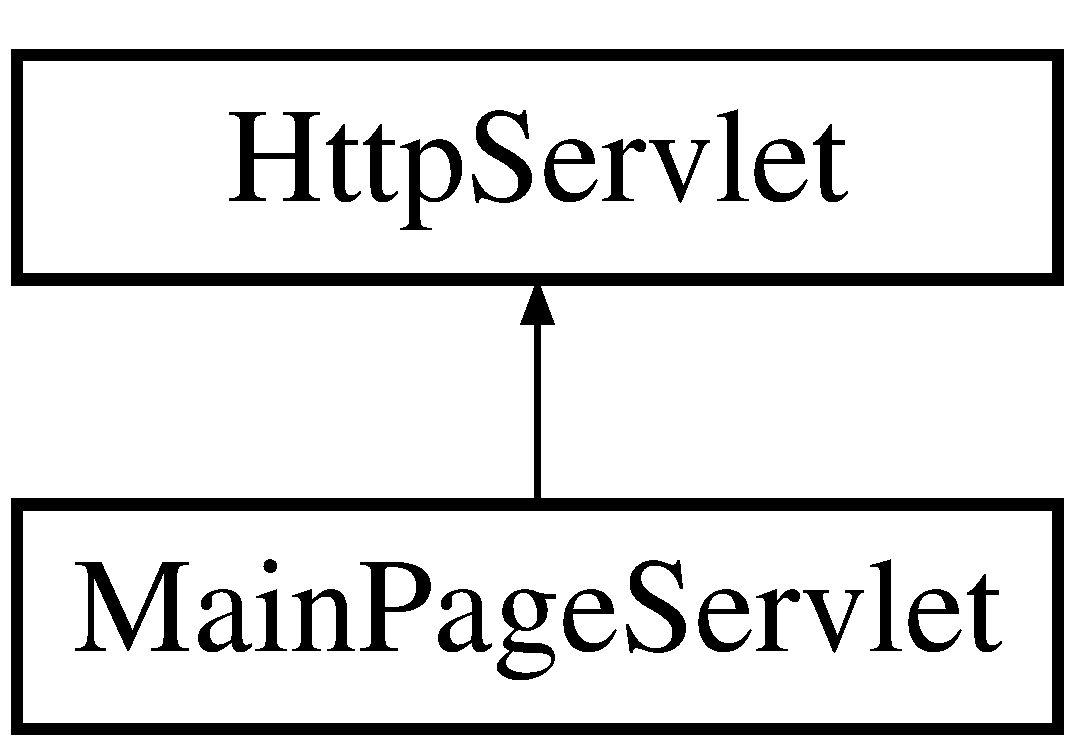
\includegraphics[height=2.000000cm]{class_main_page_servlet}
\end{center}
\end{figure}
\subsection*{Public Member Functions}
\begin{DoxyCompactItemize}
\item 
\hyperlink{class_main_page_servlet_a0b23130b80534dc206b4a288b1e53020}{Main\+Page\+Servlet} ()
\end{DoxyCompactItemize}
\subsection*{Protected Member Functions}
\begin{DoxyCompactItemize}
\item 
void \hyperlink{class_main_page_servlet_aa6d8401b0765748b6b8d02e3b83927b2}{do\+Get} (Http\+Servlet\+Request request, Http\+Servlet\+Response response)  throws Servlet\+Exception, I\+O\+Exception 
\item 
void \hyperlink{class_main_page_servlet_ac9c39a575df8e9a72cd77fa1e6f04479}{do\+Post} (Http\+Servlet\+Request request, Http\+Servlet\+Response response)  throws Servlet\+Exception, I\+O\+Exception 
\end{DoxyCompactItemize}
\subsection*{Static Protected Attributes}
\begin{DoxyCompactItemize}
\item 
\hypertarget{class_main_page_servlet_a3a18f3925a7ddd020df651e280ef6595}{}static final String {\bfseries D\+B\+\_\+\+U\+R\+L} = \char`\"{}jdbc\+:mysql\+://ec2-\/52-\/50-\/117-\/148.eu-\/west-\/1.compute.\+amazonaws.\+com/group2\+Project\char`\"{}\label{class_main_page_servlet_a3a18f3925a7ddd020df651e280ef6595}

\item 
\hypertarget{class_main_page_servlet_a352c5948af9fd48fa8802eab03d705e5}{}static final String {\bfseries D\+B\+\_\+\+U\+S\+E\+R} = \char`\"{}root\char`\"{}\label{class_main_page_servlet_a352c5948af9fd48fa8802eab03d705e5}

\item 
\hypertarget{class_main_page_servlet_a8e66c1b3040a36ce585bab821a8c2c28}{}static final String {\bfseries D\+B\+\_\+\+P\+A\+S\+S\+W\+O\+R\+D} = \char`\"{}1234\char`\"{}\label{class_main_page_servlet_a8e66c1b3040a36ce585bab821a8c2c28}

\end{DoxyCompactItemize}


\subsection{Detailed Description}
Servlet implementation class \hyperlink{class_main_page_servlet}{Main\+Page\+Servlet} 

\subsection{Constructor \& Destructor Documentation}
\hypertarget{class_main_page_servlet_a0b23130b80534dc206b4a288b1e53020}{}\index{Main\+Page\+Servlet@{Main\+Page\+Servlet}!Main\+Page\+Servlet@{Main\+Page\+Servlet}}
\index{Main\+Page\+Servlet@{Main\+Page\+Servlet}!Main\+Page\+Servlet@{Main\+Page\+Servlet}}
\subsubsection[{Main\+Page\+Servlet()}]{\setlength{\rightskip}{0pt plus 5cm}Main\+Page\+Servlet.\+Main\+Page\+Servlet (
\begin{DoxyParamCaption}
{}
\end{DoxyParamCaption}
)}\label{class_main_page_servlet_a0b23130b80534dc206b4a288b1e53020}
\begin{DoxySeeAlso}{See also}
Http\+Servlet\+::\+Http\+Servlet() 
\end{DoxySeeAlso}


\subsection{Member Function Documentation}
\hypertarget{class_main_page_servlet_aa6d8401b0765748b6b8d02e3b83927b2}{}\index{Main\+Page\+Servlet@{Main\+Page\+Servlet}!do\+Get@{do\+Get}}
\index{do\+Get@{do\+Get}!Main\+Page\+Servlet@{Main\+Page\+Servlet}}
\subsubsection[{do\+Get(\+Http\+Servlet\+Request request, Http\+Servlet\+Response response)}]{\setlength{\rightskip}{0pt plus 5cm}void Main\+Page\+Servlet.\+do\+Get (
\begin{DoxyParamCaption}
\item[{Http\+Servlet\+Request}]{request, }
\item[{Http\+Servlet\+Response}]{response}
\end{DoxyParamCaption}
) throws Servlet\+Exception, I\+O\+Exception\hspace{0.3cm}{\ttfamily [protected]}}\label{class_main_page_servlet_aa6d8401b0765748b6b8d02e3b83927b2}
\begin{DoxySeeAlso}{See also}
Http\+Servlet\+::do\+Get(\+Http\+Servlet\+Request request, Http\+Servlet\+Response response) 
\end{DoxySeeAlso}
\hypertarget{class_main_page_servlet_ac9c39a575df8e9a72cd77fa1e6f04479}{}\index{Main\+Page\+Servlet@{Main\+Page\+Servlet}!do\+Post@{do\+Post}}
\index{do\+Post@{do\+Post}!Main\+Page\+Servlet@{Main\+Page\+Servlet}}
\subsubsection[{do\+Post(\+Http\+Servlet\+Request request, Http\+Servlet\+Response response)}]{\setlength{\rightskip}{0pt plus 5cm}void Main\+Page\+Servlet.\+do\+Post (
\begin{DoxyParamCaption}
\item[{Http\+Servlet\+Request}]{request, }
\item[{Http\+Servlet\+Response}]{response}
\end{DoxyParamCaption}
) throws Servlet\+Exception, I\+O\+Exception\hspace{0.3cm}{\ttfamily [protected]}}\label{class_main_page_servlet_ac9c39a575df8e9a72cd77fa1e6f04479}
\begin{DoxySeeAlso}{See also}
Http\+Servlet\+::do\+Post(\+Http\+Servlet\+Request request, Http\+Servlet\+Response response) 
\end{DoxySeeAlso}


The documentation for this class was generated from the following file\+:\begin{DoxyCompactItemize}
\item 
src/Main\+Page\+Servlet.\+java\end{DoxyCompactItemize}

\hypertarget{class_osman_servlet}{}\section{Osman\+Servlet Class Reference}
\label{class_osman_servlet}\index{Osman\+Servlet@{Osman\+Servlet}}
Inheritance diagram for Osman\+Servlet\+:\begin{figure}[H]
\begin{center}
\leavevmode
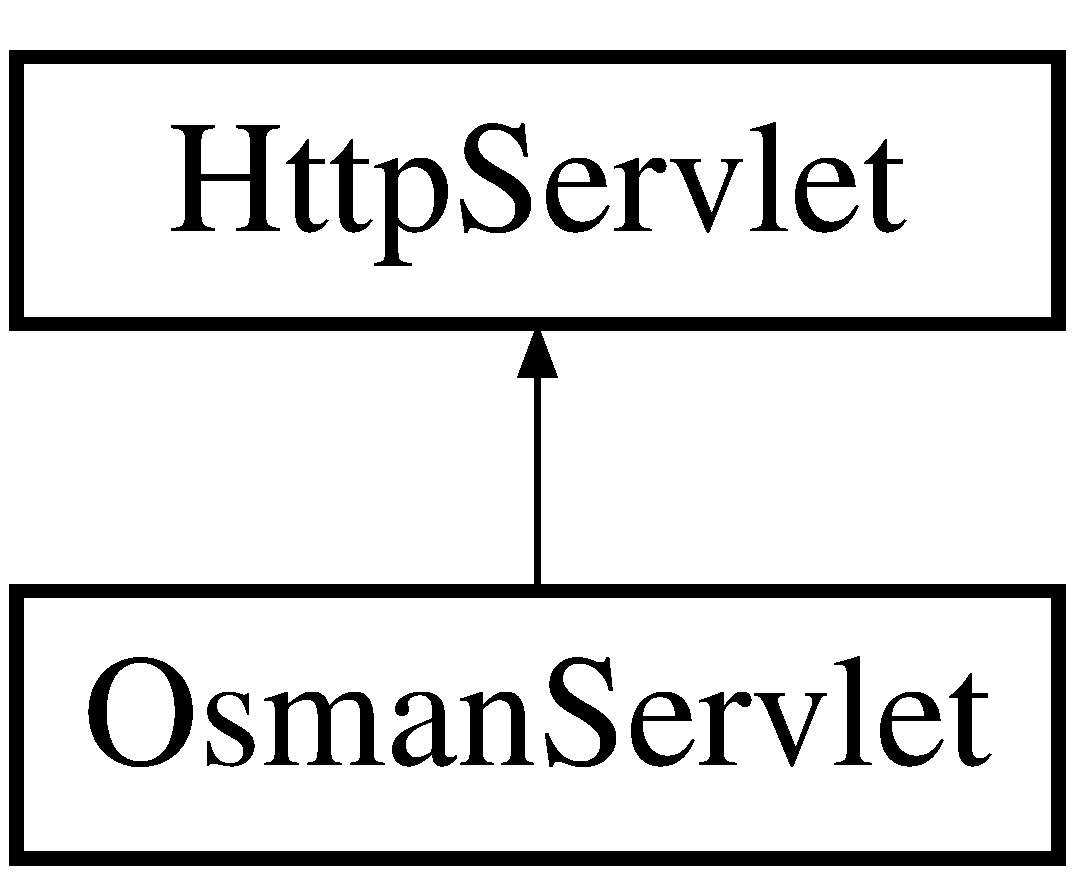
\includegraphics[height=2.000000cm]{class_osman_servlet}
\end{center}
\end{figure}
\subsection*{Public Member Functions}
\begin{DoxyCompactItemize}
\item 
\hyperlink{class_osman_servlet_a01c17538feb7733f728cab3b6be93a5b}{Osman\+Servlet} ()
\end{DoxyCompactItemize}
\subsection*{Protected Member Functions}
\begin{DoxyCompactItemize}
\item 
void \hyperlink{class_osman_servlet_aafa070b4f76cd5d88a74348cbc4f9644}{do\+Get} (Http\+Servlet\+Request request, Http\+Servlet\+Response response)  throws Servlet\+Exception, I\+O\+Exception 
\item 
void \hyperlink{class_osman_servlet_a9766ba6b1e0bc1e3277b20834c61a5e2}{do\+Post} (Http\+Servlet\+Request request, Http\+Servlet\+Response response)  throws Servlet\+Exception, I\+O\+Exception 
\end{DoxyCompactItemize}


\subsection{Detailed Description}
Servlet implementation class \hyperlink{class_osman_servlet}{Osman\+Servlet} 

\subsection{Constructor \& Destructor Documentation}
\hypertarget{class_osman_servlet_a01c17538feb7733f728cab3b6be93a5b}{}\index{Osman\+Servlet@{Osman\+Servlet}!Osman\+Servlet@{Osman\+Servlet}}
\index{Osman\+Servlet@{Osman\+Servlet}!Osman\+Servlet@{Osman\+Servlet}}
\subsubsection[{Osman\+Servlet()}]{\setlength{\rightskip}{0pt plus 5cm}Osman\+Servlet.\+Osman\+Servlet (
\begin{DoxyParamCaption}
{}
\end{DoxyParamCaption}
)}\label{class_osman_servlet_a01c17538feb7733f728cab3b6be93a5b}
\begin{DoxySeeAlso}{See also}
Http\+Servlet\+::\+Http\+Servlet() 
\end{DoxySeeAlso}


\subsection{Member Function Documentation}
\hypertarget{class_osman_servlet_aafa070b4f76cd5d88a74348cbc4f9644}{}\index{Osman\+Servlet@{Osman\+Servlet}!do\+Get@{do\+Get}}
\index{do\+Get@{do\+Get}!Osman\+Servlet@{Osman\+Servlet}}
\subsubsection[{do\+Get(\+Http\+Servlet\+Request request, Http\+Servlet\+Response response)}]{\setlength{\rightskip}{0pt plus 5cm}void Osman\+Servlet.\+do\+Get (
\begin{DoxyParamCaption}
\item[{Http\+Servlet\+Request}]{request, }
\item[{Http\+Servlet\+Response}]{response}
\end{DoxyParamCaption}
) throws Servlet\+Exception, I\+O\+Exception\hspace{0.3cm}{\ttfamily [protected]}}\label{class_osman_servlet_aafa070b4f76cd5d88a74348cbc4f9644}
\begin{DoxySeeAlso}{See also}
Http\+Servlet\+::do\+Get(\+Http\+Servlet\+Request request, Http\+Servlet\+Response response) 
\end{DoxySeeAlso}
\hypertarget{class_osman_servlet_a9766ba6b1e0bc1e3277b20834c61a5e2}{}\index{Osman\+Servlet@{Osman\+Servlet}!do\+Post@{do\+Post}}
\index{do\+Post@{do\+Post}!Osman\+Servlet@{Osman\+Servlet}}
\subsubsection[{do\+Post(\+Http\+Servlet\+Request request, Http\+Servlet\+Response response)}]{\setlength{\rightskip}{0pt plus 5cm}void Osman\+Servlet.\+do\+Post (
\begin{DoxyParamCaption}
\item[{Http\+Servlet\+Request}]{request, }
\item[{Http\+Servlet\+Response}]{response}
\end{DoxyParamCaption}
) throws Servlet\+Exception, I\+O\+Exception\hspace{0.3cm}{\ttfamily [protected]}}\label{class_osman_servlet_a9766ba6b1e0bc1e3277b20834c61a5e2}
\begin{DoxySeeAlso}{See also}
Http\+Servlet\+::do\+Post(\+Http\+Servlet\+Request request, Http\+Servlet\+Response response) 
\end{DoxySeeAlso}


The documentation for this class was generated from the following file\+:\begin{DoxyCompactItemize}
\item 
src/Osman\+Servlet.\+java\end{DoxyCompactItemize}

\hypertarget{class_yigit_servlet}{}\section{Yigit\+Servlet Class Reference}
\label{class_yigit_servlet}\index{Yigit\+Servlet@{Yigit\+Servlet}}
Inheritance diagram for Yigit\+Servlet\+:\begin{figure}[H]
\begin{center}
\leavevmode
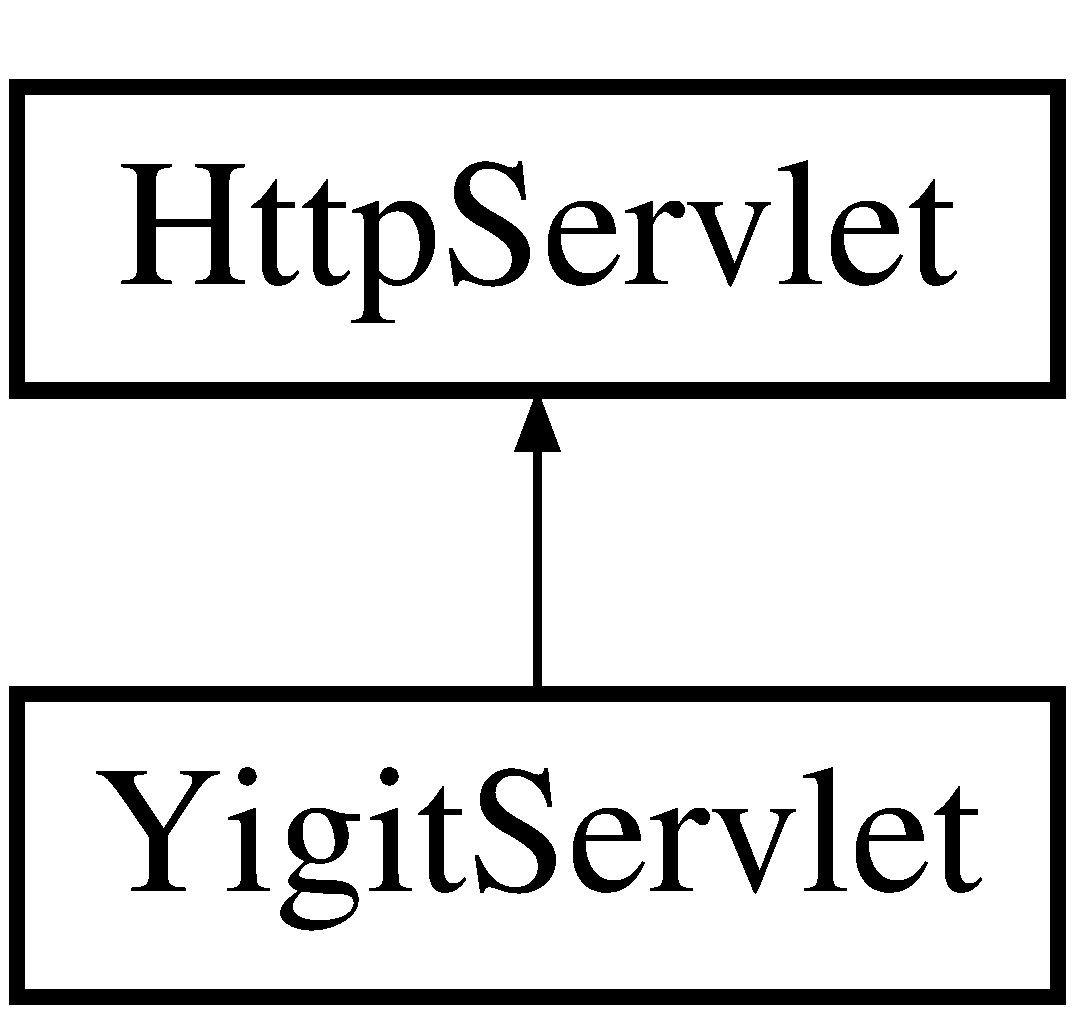
\includegraphics[height=2.000000cm]{class_yigit_servlet}
\end{center}
\end{figure}
\subsection*{Public Member Functions}
\begin{DoxyCompactItemize}
\item 
\hyperlink{class_yigit_servlet_a2cf35716343b40ed5d31bc20bd0e4281}{Yigit\+Servlet} ()
\end{DoxyCompactItemize}
\subsection*{Protected Member Functions}
\begin{DoxyCompactItemize}
\item 
Connection \hyperlink{class_yigit_servlet_afbf5525cf34aecfbc5c2d7c0a5398d45}{establish\+Database} ()
\item 
String \hyperlink{class_yigit_servlet_a03f680ab69c811ba4bb6024bb172c783}{get\+Query} ()  throws Unsupported\+Encoding\+Exception
\item 
void \hyperlink{class_yigit_servlet_a67dcab9984048772508f806eec206392}{initialize\+Parameters} (Http\+Servlet\+Request request)
\item 
J\+S\+O\+N\+Array \hyperlink{class_yigit_servlet_acb708f5a65546d97991965287c3f226d}{get\+Movies} ()
\item 
void \hyperlink{class_yigit_servlet_a87f5660fd804020140513bfd608a1fad}{do\+Get} (Http\+Servlet\+Request request, Http\+Servlet\+Response response)  throws I\+O\+Exception  
\item 
void \hyperlink{class_yigit_servlet_a6b23eda49b2fe7abb63786c20fe01d75}{do\+Post} (Http\+Servlet\+Request request, Http\+Servlet\+Response response)  throws Servlet\+Exception, I\+O\+Exception 
\end{DoxyCompactItemize}


\subsection{Detailed Description}
Servlet implementation class \hyperlink{class_yigit_servlet}{Yigit\+Servlet} 

\subsection{Constructor \& Destructor Documentation}
\hypertarget{class_yigit_servlet_a2cf35716343b40ed5d31bc20bd0e4281}{}\index{Yigit\+Servlet@{Yigit\+Servlet}!Yigit\+Servlet@{Yigit\+Servlet}}
\index{Yigit\+Servlet@{Yigit\+Servlet}!Yigit\+Servlet@{Yigit\+Servlet}}
\subsubsection[{Yigit\+Servlet()}]{\setlength{\rightskip}{0pt plus 5cm}Yigit\+Servlet.\+Yigit\+Servlet (
\begin{DoxyParamCaption}
{}
\end{DoxyParamCaption}
)}\label{class_yigit_servlet_a2cf35716343b40ed5d31bc20bd0e4281}
Constructor of the class \begin{DoxySeeAlso}{See also}
Http\+Servlet\+::\+Http\+Servlet() 
\end{DoxySeeAlso}


\subsection{Member Function Documentation}
\hypertarget{class_yigit_servlet_a87f5660fd804020140513bfd608a1fad}{}\index{Yigit\+Servlet@{Yigit\+Servlet}!do\+Get@{do\+Get}}
\index{do\+Get@{do\+Get}!Yigit\+Servlet@{Yigit\+Servlet}}
\subsubsection[{do\+Get(\+Http\+Servlet\+Request request, Http\+Servlet\+Response response)}]{\setlength{\rightskip}{0pt plus 5cm}void Yigit\+Servlet.\+do\+Get (
\begin{DoxyParamCaption}
\item[{Http\+Servlet\+Request}]{request, }
\item[{Http\+Servlet\+Response}]{response}
\end{DoxyParamCaption}
) throws I\+O\+Exception\hspace{0.3cm}{\ttfamily [protected]}}\label{class_yigit_servlet_a87f5660fd804020140513bfd608a1fad}

\begin{DoxyExceptions}{Exceptions}
{\em I\+O\+Exception} & \\
\hline
\end{DoxyExceptions}
\begin{DoxySeeAlso}{See also}
Http\+Servlet\+::do\+Get(\+Http\+Servlet\+Request request, Http\+Servlet\+Response response) 
\end{DoxySeeAlso}
\hypertarget{class_yigit_servlet_a6b23eda49b2fe7abb63786c20fe01d75}{}\index{Yigit\+Servlet@{Yigit\+Servlet}!do\+Post@{do\+Post}}
\index{do\+Post@{do\+Post}!Yigit\+Servlet@{Yigit\+Servlet}}
\subsubsection[{do\+Post(\+Http\+Servlet\+Request request, Http\+Servlet\+Response response)}]{\setlength{\rightskip}{0pt plus 5cm}void Yigit\+Servlet.\+do\+Post (
\begin{DoxyParamCaption}
\item[{Http\+Servlet\+Request}]{request, }
\item[{Http\+Servlet\+Response}]{response}
\end{DoxyParamCaption}
) throws Servlet\+Exception, I\+O\+Exception\hspace{0.3cm}{\ttfamily [protected]}}\label{class_yigit_servlet_a6b23eda49b2fe7abb63786c20fe01d75}
\begin{DoxySeeAlso}{See also}
Http\+Servlet\+::do\+Post(\+Http\+Servlet\+Request request, Http\+Servlet\+Response response) 
\end{DoxySeeAlso}
\hypertarget{class_yigit_servlet_afbf5525cf34aecfbc5c2d7c0a5398d45}{}\index{Yigit\+Servlet@{Yigit\+Servlet}!establish\+Database@{establish\+Database}}
\index{establish\+Database@{establish\+Database}!Yigit\+Servlet@{Yigit\+Servlet}}
\subsubsection[{establish\+Database()}]{\setlength{\rightskip}{0pt plus 5cm}Connection Yigit\+Servlet.\+establish\+Database (
\begin{DoxyParamCaption}
{}
\end{DoxyParamCaption}
)\hspace{0.3cm}{\ttfamily [protected]}}\label{class_yigit_servlet_afbf5525cf34aecfbc5c2d7c0a5398d45}
Creates the database connection using the credentials defined in main\+Page\+Servlet. Checks the class and the S\+Q\+L availability \begin{DoxyReturn}{Returns}
The database connection object 
\end{DoxyReturn}
\hypertarget{class_yigit_servlet_acb708f5a65546d97991965287c3f226d}{}\index{Yigit\+Servlet@{Yigit\+Servlet}!get\+Movies@{get\+Movies}}
\index{get\+Movies@{get\+Movies}!Yigit\+Servlet@{Yigit\+Servlet}}
\subsubsection[{get\+Movies()}]{\setlength{\rightskip}{0pt plus 5cm}J\+S\+O\+N\+Array Yigit\+Servlet.\+get\+Movies (
\begin{DoxyParamCaption}
{}
\end{DoxyParamCaption}
)\hspace{0.3cm}{\ttfamily [protected]}}\label{class_yigit_servlet_acb708f5a65546d97991965287c3f226d}
This method uses sparql query service and gets the query result data, then exports to J\+S\+O\+N and returns the J\+S\+O\+N Array of the Movies that are found from the query \begin{DoxyReturn}{Returns}

\end{DoxyReturn}
\hypertarget{class_yigit_servlet_a03f680ab69c811ba4bb6024bb172c783}{}\index{Yigit\+Servlet@{Yigit\+Servlet}!get\+Query@{get\+Query}}
\index{get\+Query@{get\+Query}!Yigit\+Servlet@{Yigit\+Servlet}}
\subsubsection[{get\+Query()}]{\setlength{\rightskip}{0pt plus 5cm}String Yigit\+Servlet.\+get\+Query (
\begin{DoxyParamCaption}
{}
\end{DoxyParamCaption}
) throws Unsupported\+Encoding\+Exception\hspace{0.3cm}{\ttfamily [protected]}}\label{class_yigit_servlet_a03f680ab69c811ba4bb6024bb172c783}
Store the main query String for modularity \begin{DoxyReturn}{Returns}
the query string with the right encoding 
\end{DoxyReturn}

\begin{DoxyExceptions}{Exceptions}
{\em Unsupported\+Encoding\+Exception} & \\
\hline
\end{DoxyExceptions}
\hypertarget{class_yigit_servlet_a67dcab9984048772508f806eec206392}{}\index{Yigit\+Servlet@{Yigit\+Servlet}!initialize\+Parameters@{initialize\+Parameters}}
\index{initialize\+Parameters@{initialize\+Parameters}!Yigit\+Servlet@{Yigit\+Servlet}}
\subsubsection[{initialize\+Parameters(\+Http\+Servlet\+Request request)}]{\setlength{\rightskip}{0pt plus 5cm}void Yigit\+Servlet.\+initialize\+Parameters (
\begin{DoxyParamCaption}
\item[{Http\+Servlet\+Request}]{request}
\end{DoxyParamCaption}
)\hspace{0.3cm}{\ttfamily [protected]}}\label{class_yigit_servlet_a67dcab9984048772508f806eec206392}
Assigns the initial duration value which is 0 and the query limit which is 10 The structure of the method is the same since it needs to check the same exceptions with try catches. 
\begin{DoxyParams}{Parameters}
{\em request} & \\
\hline
\end{DoxyParams}


The documentation for this class was generated from the following file\+:\begin{DoxyCompactItemize}
\item 
src/Yigit\+Servlet.\+java\end{DoxyCompactItemize}

%--- End generated contents ---

% Index
\backmatter
\newpage
\phantomsection
\clearemptydoublepage
\addcontentsline{toc}{chapter}{Index}
\printindex

\end{document}
